\documentclass[border=4pt]{standalone}
% Shared style for every diagram. Colour-blind-safe palette (Okabe-Ito).
\usepackage[T1]{fontenc}
\usepackage{helvet}
\renewcommand{\familydefault}{\sfdefault}
\usepackage{tikz}
\usetikzlibrary{arrows.meta,positioning,fit,backgrounds,calc,shapes.geometric,decorations.pathreplacing}
\definecolor{cblue}{HTML}{0072B2}
\definecolor{corange}{HTML}{E69F00}
\definecolor{cgreen}{HTML}{009E73}
\definecolor{cred}{HTML}{D55E00}
\definecolor{cpurple}{HTML}{CC79A7}
\definecolor{cgrey}{HTML}{6B7280}
\definecolor{csky}{HTML}{56B4E9}
\tikzset{
  >={Stealth[length=2.2mm]},
  box/.style={draw, rounded corners=3pt, align=center, minimum height=11mm, minimum width=22mm, font=\small, line width=0.7pt},
  real/.style={box, draw=cblue, fill=cblue!8},
  sim/.style={box, draw=corange, fill=corange!12},
  future/.style={box, draw=cgrey, dashed, fill=white},
  flow/.style={->, line width=0.8pt, draw=black!75},
  dflow/.style={->, line width=0.8pt, dashed, draw=cgrey},
  lbl/.style={font=\scriptsize, text=black!70},
  group/.style={draw=black!25, rounded corners=6pt, inner sep=6pt},
}

\begin{document}
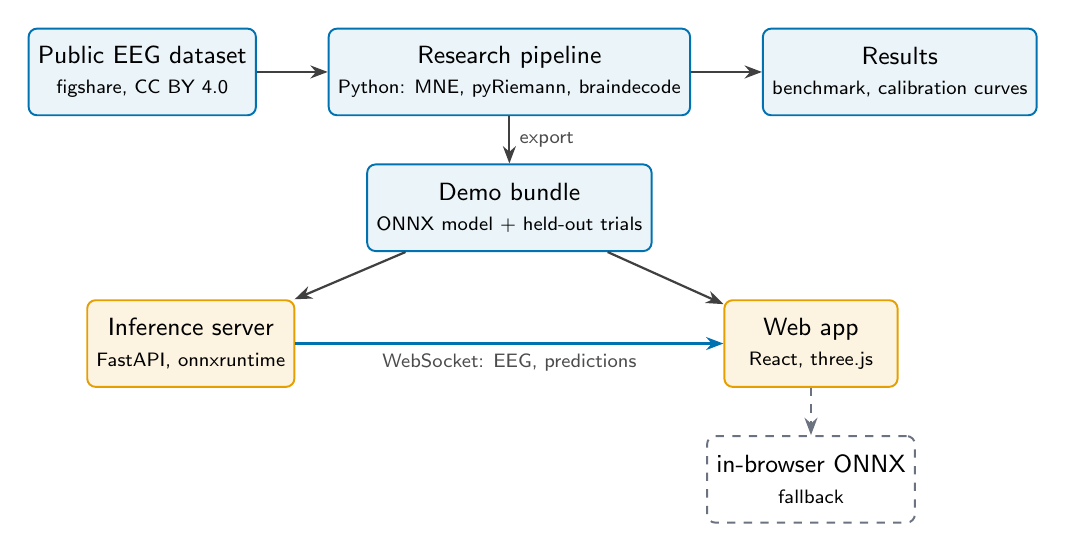
\begin{tikzpicture}[node distance=6mm and 9mm]
  \node[real] (data) {Public EEG dataset\\\scriptsize figshare, CC BY 4.0};
  \node[real, right=of data] (pipe) {Research pipeline\\\scriptsize Python: MNE, pyRiemann, braindecode};
  \node[real, right=of pipe] (res) {Results\\\scriptsize benchmark, calibration curves};
  \node[real, below=of pipe] (bundle) {Demo bundle\\\scriptsize ONNX model + held-out trials};
  \node[sim, below left=of bundle] (server) {Inference server\\\scriptsize FastAPI, onnxruntime};
  \node[sim, below right=of bundle] (web) {Web app\\\scriptsize React, three.js};
  \node[future, below=of web] (ort) {in-browser ONNX\\\scriptsize fallback};
  \draw[flow] (data) -- (pipe); \draw[flow] (pipe) -- (res); \draw[flow] (pipe) -- node[lbl, right] {export} (bundle);
  \draw[flow] (bundle) -- (server); \draw[flow] (bundle) -- (web);
  \draw[flow, cblue] (server) -- node[lbl, below] {WebSocket: EEG, predictions} (web);
  \draw[dflow] (web) -- (ort);
\end{tikzpicture}
\end{document}
